\documentclass[11pt, oneside]{article}   	% use "amsart" instead of "article" for AMSLaTeX format
\usepackage{geometry}                		% See geometry.pdf to learn the layout options. There are lots.
\geometry{a4paper}                   		% ... or a4paper or a5paper or ... 
%\geometry{landscape}                		% Activate for rotated page geometry
%\usepackage[parfill]{parskip}    		% Activate to begin paragraphs with an empty line rather than an indent
\usepackage{graphicx}				% Use pdf, png, jpg, or eps§ with pdflatex; use eps in DVI mode
								% TeX will automatically convert eps --> pdf in pdflatex		
\usepackage{amssymb,amsmath}


% Tikz packages
\usepackage{float}
\usepackage{pgfplots}
\usepackage{tikz}
\usepackage{tikzsymbols}
\pgfplotsset{compat=1.15}

% Line thickness. One might want to multiply these values by 1.5 to make sure they are not too thin for printing!
\tikzset{
    ultra thin/.style= {line width=0.1pt},
    very thin/.style=  {line width=0.2pt},
    thin/.style=       {line width=0.4pt},% thin is the default line
    semithick/.style=  {line width=0.6pt},
    thick/.style=      {line width=0.8pt},
    very thick/.style= {line width=1.2pt},
    ultra thick/.style={line width=1.6pt}
}
\tikzset{every picture/.style={thin}} %or use: "`line width=1 pt,"<-- note:if you write line width, you must use a value with unit
\pgfplotsset{every axis/.append style={thin, grid style={thin,}, tick style={very thin,}}}

% Colors
\definecolor{ultikzblue}{rgb}{0.00000,0.44700,0.74100}%
\definecolor{ultikzred}{rgb}{0.85000,0.32500,0.09800}%
\definecolor{ultikzyellow}{rgb}{0.92900,0.69400,0.12500}%
\definecolor{ultikzpurple}{rgb}{0.49400,0.18400,0.55600}%
\definecolor{ultikzgreen}{rgb}{0.46600,0.67400,0.18800}%
\definecolor{ultikzburgundy}{rgb}{0.63500,0.07800,0.18400}%

\title{Ultimate TikZ Figures for Publications}
\author{Slobodan Milovanovi\'c}
%\date{}							% Activate to display a given date or no date

\begin{document}
\maketitle
%
%
%
\section{Line Plots}
Here is an example of a standard line plot with a legend.
%
\begin{figure}[H]
\centering
\input{ultikz/lineplots_basic.tikz}
\caption{\emph{Examples of GAs with different shape parameter values and PHSs of different degrees.}}
\label{fig:RBF}
\end{figure}
%
%
\subsection{Logarithmic Line Plots}
This is an example combining two logarithmic line plots with different mark symbols.
\begin{figure}[H]
\centering
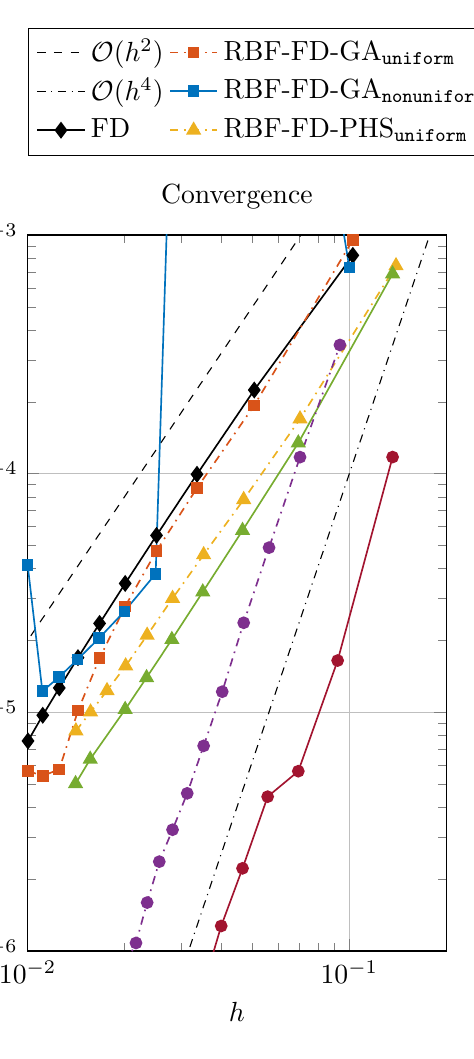
\begin{tikzpicture}[trim axis left, trim axis right, baseline]
  \begin{axis}[
  grid=major,
  width=0.4383\textwidth,
  height=0.75\textwidth,
  at={(0\textwidth,0\textwidth)},
  scale only axis,
  unbounded coords=jump,
  % x axis
  xmode=log, %this triggers the log scale
  xmin=1e-02,
  xmax=2e-01,
  xlabel={$h$},
  xminorticks=true,
  % y axis
  ymode=log,
  ymin=1e-06,
  ymax=1e-03,
  yminorticks=true,
  ytick distance=10^1, %this sets the tick distance
  ylabel={$\Delta u_{\max}$},
  %title style={font=\bfseries}, % uncomment for bold title
  title={Convergence},
  legend columns=3,
  transpose legend,
  legend style={legend cell align=left, align=left, at={(0,1.2)}, anchor=west}
  ]

  \addplot [color=black, thin, dashed]
    table[row sep=crcr, y expr=\thisrow{Y}*2]{%
    X Y\\
  0.001	1e-07\\
  0.00125892541179417	1.58489319246111e-07\\
  0.00158489319246111	2.51188643150958e-07\\
  0.00199526231496888	3.98107170553497e-07\\
  0.00251188643150958	6.30957344480193e-07\\
  0.00316227766016838	1e-06\\
  0.00398107170553497	1.58489319246111e-06\\
  0.00501187233627272	2.51188643150958e-06\\
  0.00630957344480193	3.98107170553497e-06\\
  0.00794328234724281	6.30957344480193e-06\\
  0.01	1e-05\\
  0.0125892541179417	1.58489319246111e-05\\
  0.0158489319246111	2.51188643150958e-05\\
  0.0199526231496888	3.98107170553497e-05\\
  0.0251188643150958	6.30957344480194e-05\\
  0.0316227766016838	0.0001\\
  0.0398107170553497	0.000158489319246111\\
  0.0501187233627272	0.000251188643150958\\
  0.0630957344480193	0.000398107170553497\\
  0.0794328234724281	0.000630957344480193\\
  0.1	0.001\\
  0.125892541179417	0.00158489319246111\\
  0.158489319246111	0.00251188643150958\\
  0.199526231496888	0.00398107170553497\\
  0.251188643150958	0.00630957344480193\\
  0.316227766016838	0.01\\
  0.398107170553497	0.0158489319246111\\
  0.501187233627272	0.0251188643150958\\
  0.630957344480193	0.0398107170553497\\
  0.794328234724281	0.0630957344480193\\
  1	0.1\\
  };
  \addlegendentry{$\mathcal{O}(h^2)$}

  \addplot [color=black, thin, dashdotted]
    table[row sep=crcr]{%
  0.001	1e-12\\
  0.00125892541179417	2.51188643150958e-12\\
  0.00158489319246111	6.30957344480194e-12\\
  0.00199526231496888	1.58489319246111e-11\\
  0.00251188643150958	3.98107170553497e-11\\
  0.00316227766016838	1e-10\\
  0.00398107170553497	2.51188643150958e-10\\
  0.00501187233627272	6.30957344480194e-10\\
  0.00630957344480193	1.58489319246111e-09\\
  0.00794328234724281	3.98107170553497e-09\\
  0.01	1e-08\\
  0.0125892541179417	2.51188643150958e-08\\
  0.0158489319246111	6.30957344480194e-08\\
  0.0199526231496888	1.58489319246111e-07\\
  0.0251188643150958	3.98107170553498e-07\\
  0.0316227766016838	1e-06\\
  0.0398107170553497	2.51188643150958e-06\\
  0.0501187233627272	6.30957344480193e-06\\
  0.0630957344480193	1.58489319246111e-05\\
  0.0794328234724281	3.98107170553497e-05\\
  0.1	0.0001\\
  0.125892541179417	0.000251188643150958\\
  0.158489319246111	0.000630957344480193\\
  0.199526231496888	0.00158489319246111\\
  0.251188643150958	0.00398107170553497\\
  0.316227766016838	0.01\\
  0.398107170553497	0.0251188643150958\\
  0.501187233627272	0.0630957344480193\\
  0.630957344480193	0.158489319246111\\
  0.794328234724281	0.398107170553497\\
  1	1\\
  };
  \addlegendentry{$\mathcal{O}(h^4)$}

  \addplot [color=black, semithick, mark=diamond*, mark options={scale = 1.3, solid, black}]
    table[row sep=crcr]{%
    0.0100250626566416	7.5886574535161e-06\\
    0.011142061281337	9.72228147643741e-06\\
    0.0125391849529781	1.26596809826227e-05\\
    0.014336917562724	1.69486755397803e-05\\
    0.0167364016736402	2.35866771239822e-05\\
    0.0201005025125628	3.46796687033725e-05\\
    0.0251572327044025	5.51237913711251e-05\\
    0.0336134453781513	9.94080377643199e-05\\
    0.0506329113924051	0.000224138718419901\\
    0.102564102564103	0.000821697635051559\\
  };
  \addlegendentry{$\text{FD}$}

  \addplot [color=ultikzred, semithick, dashdotted, mark=square*, mark options={scale = 0.9,solid, ultikzred}]
    table[row sep=crcr]{%
    0.0100250626566416	5.67489189767789e-06\\
  0.011142061281337	5.4245897675026e-06\\
  0.0125391849529781	5.76537132542312e-06\\
  0.014336917562724	1.01673887758155e-05\\
  0.0167364016736402	1.68818812815268e-05\\
  0.0201005025125628	2.78000505424987e-05\\
  0.0251572327044025	4.74942057093787e-05\\
  0.0336134453781513	8.70798482893939e-05\\
  0.0506329113924051	0.000193301090642285\\
  0.102564102564103	0.000954288395106928\\
  };
  \addlegendentry{$\text{RBF-FD-GA}_{\texttt{uniform}}$}

  \addplot [color=ultikzblue, semithick, mark=square*, mark options={scale = 0.9, solid, ultikzblue}]
    table[row sep=crcr]{%
    0.01	4.14165843865555e-05\\
  0.0111111111111111	1.22566457229217e-05\\
  0.0125	1.40298458809716e-05\\
  0.0142857142857143	1.664986889751e-05\\
  0.0166666666666667	2.04396388880333e-05\\
  0.02	2.64971538777616e-05\\
  0.025	3.80636671498055e-05\\
  0.0333333333333333	6.40359806
  0.05	0.000153151719320656\\
  0.1	0.000730421951017157\\
  };
  \addlegendentry{$\text{RBF-FD-GA}_{\texttt{nonuniform}}$}

  \addplot [color=ultikzyellow, semithick, dashdotted, mark=triangle*, mark options={scale = 1.3,solid, ultikzyellow}]
    table[row sep=crcr]{%
    0.014124491030929	8.36410001815724e-06\\
  0.0156917051052617	1.0028502564801e-05\\
  0.0176501127404552	1.23307428878117e-05\\
  0.0201670703622372	1.56518944708431e-05\\
  0.0235212743230775	2.10393559688313e-05\\
  0.0282138246343439	3.00189176842408e-05\\
  0.0352453688425121	4.57511141431395e-05\\
  0.046945252681302	7.78916616573505e-05\\
  0.0702728368926307	0.000169616596950958\\
  0.139686059153916	0.000743167977149496\\
  };
  \addlegendentry{$\text{RBF-FD-PHS}_{\texttt{uniform}}$}

  \addplot [color=ultikzgreen, semithick, mark=triangle*, mark options={scale = 1.3,solid, ultikzgreen}]
    table[row sep=crcr]{%
    0.0140893116711202	5.02720013236327e-06\\
  0.0156482978157298	6.36362730365575e-06
  0.0175952133454409	7.93251233059677e-06\\
  0.0200954286780432	1.02810154664346e-05\\
  0.0234238773236666	1.39793874041304e-05\\
  0.028073804789235	2.01883525170823e-05\\
  0.0350271291661823	3.19452679388398e-05\\
  0.046558865430144	5.78232547853892e-05\\
  0.0694105608393805	0.000134546330187221\\
  0.136319635318199	0.000687264699283568\\
  };
  \addlegendentry{$\text{RBF-FD-PHS}_{\texttt{nonuniform}}$}

  \addplot [color=ultikzpurple, semithick, dashdotted, mark=*, mark options={solid, ultikzpurple}]
    table[row sep=crcr]{%
  0.0201670703622372	8.86676792243582e-07\\
  0.0217154113994819	1.08094053489867e-06\\
  0.0235212743230775	1.59605544365503e-06\\
  0.0256547337551516	2.36856397064627e-06\\
  0.0282138246343439	3.22326044284102e-06\\
  0.0313400329814846	4.57864276742076e-06\\
  0.0352453688425121	7.23881122826828e-06\\
  0.0402625627785849	1.22034416352584e-05\\
  0.046945252681302	2.37328354763949e-05\\
  0.0562878035784234	4.89880039680132e-05\\
  0.0702728368926307	0.000117282713859648\\
  0.0935049164424369	0.000346118628974414\\
  };
  \addlegendentry{$\text{RBF-FD-PHS}^{\texttt{smoothed}}_{\texttt{uniform}}$}

  \addplot [color=ultikzburgundy, semithick, mark=*, mark options={solid, ultikzburgundy}]
    table[row sep=crcr]{%
    0.0350271291661823	6.99972089132939e-07\\
    0.0399780181333785	1.27354519761577e-06\\
    0.046558865430144	2.22068321180727e-06\\
    0.0557332304127295	4.43330995397034e-06\\
    0.0694105608393805	5.66874455900854e-06\\
    0.0919844099636548	1.64849648476599e-05\\
    0.136319635318199	0.000117373463206207\\
  };
  \addlegendentry{$\text{RBF-FD-PHS}^{\texttt{smoothed}}_{\texttt{nonuniform}}$}
\end{axis}
\end{tikzpicture}%

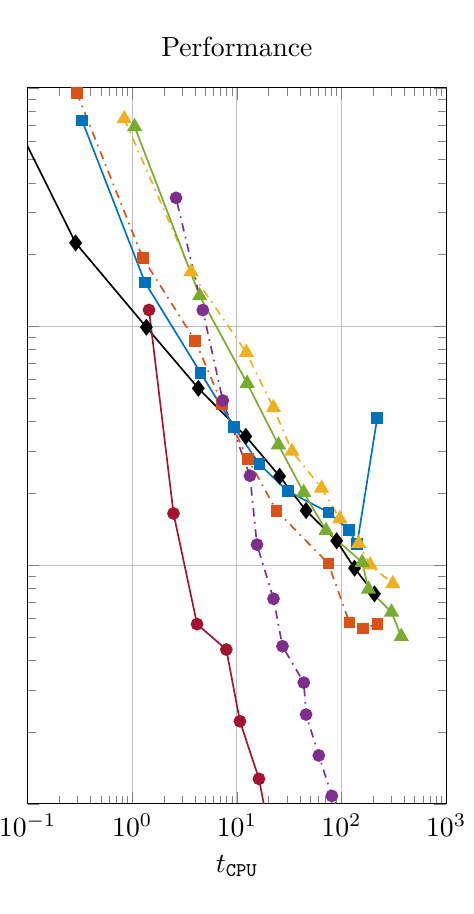
\begin{tikzpicture}[trim axis left, trim axis right, baseline]
  \begin{axis}[
  grid=major,
  width=0.4383\textwidth,
  height=0.75\textwidth,
  at={(0\textwidth,0\textwidth)},
  scale only axis,
  unbounded coords=jump,%
%x axis
  xmode=log,
  xmin=1e-01,
  xmax=1000,
  xlabel={$t_\texttt{CPU}$},%
%y axis
  ymode=log,
  ymin=1e-06,
  ymax=1e-03,
  yticklabels={,,}, %hides y ticks
  yminorticks=true,
  ytick distance=10^1,
  xminorticks=true,
  xmajorgrids,
  % xminorgrids,
  ymajorgrids,
  % yminorgrids,
  %ylabel={$\Delta u$},
  axis background/.style={fill=white},
  %title style={font=\bfseries},
  title={{\color{white}g} Performance {\color{white}g}},
  legend pos=north east,
  legend style={legend cell align=left,align=left}
  ]
  \addplot [color=black, semithick, mark=diamond*, mark options={scale = 1.3, solid, black}]
    table[row sep=crcr]{%
    0.06582786	0.000821697635051559\\
    0.287278344	0.000224138718419901\\
    1.363033105	9.94080377643199e-05\\
    4.280939024	5.51237913711251e-05\\
    12.175330572	3.46796687033725e-05\\
    25.616239575	2.35866771239822e-05\\
    45.866742939	1.69486755397803e-05\\
    89.876309784	1.26596809826227e-05\\
    133.115589004	9.72228147643741e-06\\
    206.569398646	7.5886574535161e-06\\
  };
  \addlegendentry{fd2}

  \addplot [color=ultikzred, semithick, dashdotted, mark=square*, mark options={scale = 0.9, solid, ultikzred}]
    table[row sep=crcr]{%
    0.294333181	0.000954288395106928\\
    1.264234185	0.000193301090642285\\
    4.002661134	8.70798482893939e-05\\
    7.21062104	4.74942057093787e-05\\
    12.789741194	2.78000505424987e-05\\
    23.987790138	1.68818812815268e-05\\
    74.876368296	1.01673887758155e-05\\
    118.737986566	5.76537132542312e-06\\
    160.362616102	5.4245897675026e-06\\
    220.215181191	5.67489189767789e-06\\
  };
  \addlegendentry{gs reg}

  \addplot [color=ultikzblue, semithick, mark=square*, mark options={scale = 0.9, solid, ultikzblue}]
    table[row sep=crcr]{%
    0.331154439	0.000730421951017157\\
    1.321707978	0.000153151719320656\\
    4.492199157	6.40359806401113e-05\\
    9.359380277	3.80636671498055e-05\\
    16.399435412	2.64971538777616e-05\\
    30.67468922	2.04396388880333e-05\\
    75.199079076	1.664986889751e-05\\
    117.664701023	1.40298458809716e-05\\
    140.823239139	1.22566457229217e-05\\
    219.44733059	4.14165843865555e-05\\
  };
  \addlegendentry{gs adap}

  \addplot [color=ultikzyellow, semithick, dashdotted, mark=triangle*, mark options={scale = 1.3,solid, ultikzyellow}]
    table[row sep=crcr]{%
    0.837605647	0.000743167977149496\\
  3.639769825	0.000169616596950958\\
  12.290603411	7.78916616573505e-05\\
  22.358980677	4.57511141431395e-05\\
  33.609578206	3.00189176842408e-05\\
  64.471801581	2.10393559688313e-05\\
  96.176644434	1.56518944708431e-05\\
  145.624530492	1.23307428878117e-05\\
  187.614598032	1.0028502564801e-05\\
  309.252198757	8.36410001815724e-06\\
  };
  \addlegendentry{phs reg}

  \addplot [color=ultikzgreen, semithick, mark=triangle*, mark options={scale = 1.3,solid, ultikzgreen}]
    table[row sep=crcr]{%
    1.053425471	0.000687264699283568\\
    4.408053073	0.000134546330187221\\
    12.539242522	5.78232547853892e-05\\
    24.935753374	3.19452679388398e-05\\
    43.468228217	2.01883525170823e-05\\
    71.169584803	1.39793874041304e-05\\
    157.613770699	1.02810154664346e-05\\
    181.066750603	7.93251233059677e-06\\
    300.717458059	6.36362730365575e-06\\
    372.861778238	5.02720013236327e-06\\
  };
  \addlegendentry{phs adap}

  \addplot [color=ultikzpurple, semithick, dashdotted, mark=*, mark options={solid, ultikzpurple}]
    table[row sep=crcr]{%
    100.308480392	8.86676792243582e-07\\
    80.801123362	1.08094053489867e-06\\
    60.677620782	1.59605544365503e-06\\
    45.861328437	2.36856397064627e-06\\
    43.590460923	3.22326044284102e-06\\
    27.272527995	4.57864276742076e-06\\
    22.378082203	7.23881122826828e-06\\
    15.556166938	1.22034416352584e-05\\
    13.325419311	2.37328354763949e-05\\
    7.335637489	4.89880039680132e-05\\
    4.719910087	0.000117282713859648\\
    2.619557301	0.000346118628974414\\
  };
  \addlegendentry{phs reg smoothed}

  \addplot [color=ultikzburgundy, semithick, mark=*, mark options={solid, ultikzburgundy}]
    table[row sep=crcr]{%
    1.444674318	0.000117373463206207\\
    2.478047665	1.64849648476599e-05\\
    4.160072468	5.66874455900854e-06\\
    7.925728684	4.43330995397034e-06\\
    10.689505454	2.22068321180727e-06\\
    16.261363834	1.27354519761577e-06\\
    21.123572908	6.99972089132939e-07\\
  };
  \addlegendentry{phs adap smoothed}
  \legend{};
\end{axis}
\end{tikzpicture}%

\caption{\emph{Convergence and computational performance.}}
\label{fig:log}
\end{figure}
%
\subsection{Custom Ticks}
%
\begin{figure}[H]
\centering
\input{ultikz/lineplots_customticks.tikz}
\caption{\emph{Examples of GAs with different shape parameter values and PHSs of different degrees.}}
\label{fig:payoff}
\end{figure}
%
%
%
\newpage
\section{Scatter Plots}
Here is an example of a scatter plot.
\begin{figure}[H]
\centering
\input{ultikz/scatterplot_basic.tikz}
\caption{\emph{A node layout.}}
\label{fig:stencils}
\end{figure}

\subsection{Different Dimensions}
\begin{figure}[H]
\centering
\input{ultikz/scatterplot_1D.tikz}\\
\vspace{11pt}
\input{ultikz/scatterplot_2D.tikz}\\
\vspace{11pt}
\input{ultikz/scatterplot_3D.tikz}\\
\caption{\emph{Equidistant Cartesian grid based node layouts for pricing options with a different number of underlying assets. The close-field boundary conditions are enforced in the blue triangle node, and the far-field boundary conditions are enforced in the red square nodes.}}
\label{fig:gridreg}
\end{figure}

\newpage
\section{Embedded Bitmap}
Color plots are usually not so easy to make in tikz, but they can be easily embedded in TikZ axes as bitmap images. 
\begin{figure}[H]
\centering
\begin{tikzpicture}[trim axis left, trim axis right, baseline]
    \begin{axis}[
        axis on top,
        grid=major,
        % the last decimal number is the width of the bitmap in pixels that allows for the figure to be scaled perfectly
        width=0.9*4*0.2000\textwidth,
        height=0.9*4*0.1125\textwidth,
        scale only axis,
        enlargelimits=false,
        xmode=log,
        xmin=1e-04,
        xmax=1e-01,
        ymode=log,
        ymin=1e-03,
        ymax=1e03,
        yminorticks=true,
        xminorticks=true,
        xlabel={$h$},
        % xticklabels={,,}, %hides y ticks
        ylabel={$\varepsilon$},
        ytick distance=10^1,
        % title={RBF-FD approximation: GA},
        ]

      \addplot graphics[xmin=1e-04, ymin=1e-03, xmax=1e-01, ymax=1e03]{ultikz/bitmap_heatmap.png}; %adds bitmap

      \addplot[black, semithick, domain=1e-04:1e-01, samples=100,]
        {0.0015/x} [every node/.style={yshift=8pt},sloped] %adds a line
              node[pos=0.75] {$\varepsilon^*(h)$}; % adds a sloped label on the line
    \end{axis}
  \end{tikzpicture}

\input{ultikz/embedded_colorbar.tikz}
\caption{\emph{The maximum absolute error $\Delta u_{\max}$ measured in the subdomain $\hat\Omega=[\frac{1}{3}K,\frac{5}{3}K]$ around the strike price $K$, as a function of $h$ and $\varepsilon$, for a one-dimensional European call option priced on an equidistant Cartesian grid with RBF-FD stencil size $n=3$. The black line shows the appropriate choice for the shape parameter. The RBF-FD approximation is performed using GA basis functions.}}
\label{fig:contour1}
\end{figure}


\end{document}  